\chapter{Resultados}
\label{chap_resultados}

\section{Estrutura experimental}

\warn{O presente capítulo apresenta a estrutura experimental efetivamente executada e os resultados preliminares da implementação computacional do modelo em \emph{R}. A análise foi aplicada à rota Santos--Roterdã e contempla tanto o cenário-base quanto análises complementares de sensibilidade econômica, ambiental, regulatória, operacional e específica para a rota de \gls{TCO}}. \warn{A interpretação dos resultados é realizada à luz do ambiente regulatório europeu, no qual o custo marginal de abatimento é comparado ao intervalo de referência $\gamma^{ref}$, permitindo avaliar a compatibilidade econômica dos cenários com o sinal de preço de carbono vigente.}}

A avaliação experimental é estruturada em torno de um cenário-base e de conjuntos complementares de análise de sensibilidade. O cenário-base corresponde à rota Santos--Roterdã, previamente definida no capítulo de método, e representa o caso de referência para comparação entre o \emph{bunker fuel} convencional e os cenários de biobunker. Sobre esse cenário são construídas variações paramétricas da fração de mistura $\alpha$, da rota de produção do biodiesel $r$, dos parâmetros econômicos e, de forma complementar, das condições operacionais agregadas da viagem.

\subsection{Cenário-base de referência}

O cenário-base de referência é definido por:

\[
(\mathbf{X}_0, r, \alpha)
\]

em que $\mathbf{X}_0$ representa o vetor operacional médio da rota Santos--Roterdã, $r \in \mathcal{S}_{bio}$ representa a rota de produção do biodiesel e $\alpha$ representa a fração mássica de biodiesel na mistura.

O domínio principal do experimento é definido por:

\[
(\alpha,r) \in [0{,}10,0{,}30] \times \mathcal{S}_{bio}
\]

com:

\[
\mathcal{S}_{bio} =
\{\text{soja},\text{sebo bovino},\text{UCO},\text{TCO}\}
\]

A fração de mistura é discretizada no conjunto:

\[
\alpha =
\{0{,}10,0{,}15,0{,}20,0{,}24,0{,}25,0{,}30\}
\]

de modo a incluir misturas regularmente espaçadas e, adicionalmente, o ponto de interesse específico \gls{B24}, já utilizado no exemplo numérico do capítulo de método.

\warn{Esse cenário-base constitui o núcleo da análise da dissertação, pois permite comparar, sob mesmas condições operacionais e mesma demanda útil da viagem, o efeito da origem do biodiesel e do aumento da fração renovável sobre consumo requerido, emissões, custo e custo marginal de abatimento}. \warn{Nesse contexto, o custo marginal de abatimento passa a ser interpretado como o preço implícito de carbono associado à substituição parcial do combustível fóssil, permitindo relacionar diretamente os resultados do modelo ao ambiente regulatório europeu.}}

\subsection{Cenários complementares de sensibilidade}

Além do cenário-base, a avaliação experimental compreende seis conjuntos complementares de sensibilidade.

O primeiro conjunto corresponde à sensibilidade econômica, na qual se variam os preços unitários do \emph{bunker fuel} e do biodiesel dentro de faixas compatíveis com a literatura e com referências de mercado. O objetivo é avaliar em que medida o diferencial de preço entre fração fóssil e fração renovável altera o custo total por viagem e o custo marginal de abatimento de carbono.

O segundo conjunto corresponde à sensibilidade ambiental, na qual se analisam variações nos fatores de emissão \gls{WTW} associados às diferentes rotas de produção do biodiesel. Essa etapa busca verificar a robustez da ordenação dos cenários quando se consideram incertezas ou variações metodológicas na literatura de ciclo de vida.

\warn{O terceiro conjunto corresponde à sensibilidade regulatória, na qual se avalia a resposta do modelo a diferentes valores de $\gamma^{ref}$, componente da família regulatória $\gamma$ representativo do sinal econômico de referência do carbono no ambiente regulatório europeu. Na implementação atual, esse parâmetro é convertido explicitamente para USD/tCO$_2$ antes da comparação com o custo marginal de abatimento. Essa análise permite identificar como a fronteira de viabilidade econômico-ambiental se desloca sob diferentes referências de preço do carbono.}

O quarto conjunto corresponde à sensibilidade operacional, na qual o vetor $\mathbf{X}$ é perturbado em torno do cenário-base. Nessa etapa, são avaliadas variações moderadas de distância total da rota, velocidade média e consumo médio agregado, com o objetivo de verificar se a hierarquia relativa entre os cenários de combustível se mantém sob mudanças plausíveis no perfil operacional.

\subsection{Setups experimentais}

\warn{A implementação em \emph{R} foi organizada em sete \emph{setups} experimentais principais.}

No \textbf{Setup 1}, realiza-se a varredura determinística completa do domínio $(\alpha,r)$ no cenário-base Santos--Roterdã. Esse experimento gera a matriz principal de resultados da dissertação e constitui a base para as comparações entre rotas de produção do biodiesel.

No \textbf{Setup 2}, realiza-se a sensibilidade econômica, mantendo fixos os parâmetros operacionais e ambientais e variando $p_b$ e $p_{bio,r}$. Essa etapa permite avaliar a estabilidade dos resultados econômicos frente a diferentes diferenciais de preço.

No \textbf{Setup 3}, realiza-se a sensibilidade ambiental, mantendo fixos os parâmetros operacionais e econômicos e variando os fatores $FE_{bio,r}^{WTW}$. Essa análise permite verificar a robustez dos ganhos ambientais estimados para cada rota de produção.

No \textbf{Setup 4}, realiza-se a sensibilidade regulatória, por meio da variação do componente $\gamma^{ref}$ no intervalo de referência adotado no modelo. Essa etapa permite mapear o conjunto de cenários potencialmente viáveis sob diferentes sinais de preço do carbono.

\warn{No \textbf{Setup 5}, realiza-se a sensibilidade operacional, perturbando $\mathbf{X}$ em torno do cenário-base. O objetivo é avaliar o efeito de mudanças operacionais plausíveis sobre a demanda útil da viagem, o consumo total requerido da mistura, o custo total, as emissões totais e o custo marginal de abatimento.}

\warn{No \textbf{Setup 6}, realizam-se caminhos de viabilidade regulatória com ampliação simultânea de $\gamma^{ref}$ e $\gamma^{comp}$, permitindo identificar em que patamares de indução regulatória surgem os primeiros cenários viáveis.}

\warn{No \textbf{Setup 7}, realiza-se sensibilidade específica para o biodiesel de \gls{TCO}, variando-se separadamente seu fator de emissão \gls{WTW} e seu preço relativo. Essa etapa busca verificar o quanto a atratividade dessa rota depende de premissas metodológicas e econômicas ainda mais incertas do que aquelas associadas às demais matérias-primas.}

\subsection{Variáveis de saída e estrutura dos resultados}

\warn{Para cada cenário simulado, o modelo gera um conjunto de variáveis de saída que estrutura a leitura dos resultados ao longo deste capítulo. Essas grandezas permitem acompanhar, de forma integrada, a demanda de combustível da viagem, o desempenho ambiental, o custo total e incremental, bem como o enquadramento de cada cenário no critério de viabilidade adotado. A Tabela~\ref{tab:variables_saida} sintetiza as principais saídas utilizadas na análise.}

\begin{table}[!ht]
\centering
\caption{\warn{Principais variáveis de saída do modelo e seu papel analítico}}
\label{tab:variables_saida}
\small
\setlength{\tabcolsep}{5pt}
\begin{tabular}{lll}
\hline
\warn{\parbox[t]{2.6cm}{\textbf{Variável}}} &
\warn{\parbox[t]{5.2cm}{\textbf{Interpretação}}} &
\warn{\parbox[t]{6.0cm}{\textbf{Papel analítico}}} \\
\hline
\warn{\parbox[t]{2.6cm}{$F_{kg}(0)$}} &
\warn{\parbox[t]{5.2cm}{consumo convencional de referência por viagem}} &
\warn{\parbox[t]{6.0cm}{define a base operacional a partir da qual se infere a demanda útil da travessia}} \\
\warn{\parbox[t]{2.6cm}{$F_{kg}(\alpha,r)$}} &
\warn{\parbox[t]{5.2cm}{consumo total requerido da mistura por viagem}} &
\warn{\parbox[t]{6.0cm}{explicita o efeito combinado do poder calorífico, da eficiência efetiva e da fração de mistura sobre a massa de combustível necessária}} \\
\warn{\parbox[t]{2.6cm}{$G(\alpha,r)$}} &
\warn{\parbox[t]{5.2cm}{emissões totais de gases de efeito estufa no escopo \gls{WTW}}} &
\warn{\parbox[t]{6.0cm}{mede o desempenho ambiental absoluto de cada cenário}} \\
\warn{\parbox[t]{2.6cm}{$C(\alpha,r)$}} &
\warn{\parbox[t]{5.2cm}{custo total por viagem, incluindo combustível e custo de \emph{compliance} do \gls{EUETS}}} &
\warn{\parbox[t]{6.0cm}{mede o desempenho econômico absoluto de cada cenário}} \\
\warn{\parbox[t]{2.6cm}{$\Delta C(\alpha,r)$}} &
\warn{\parbox[t]{5.2cm}{custo incremental em relação ao cenário convencional}} &
\warn{\parbox[t]{6.0cm}{permite identificar a penalidade ou vantagem econômica da substituição parcial do combustível fóssil}} \\
\warn{\parbox[t]{2.6cm}{$\Delta G(\alpha,r)$}} &
\warn{\parbox[t]{5.2cm}{redução absoluta de emissões em relação ao cenário convencional}} &
\warn{\parbox[t]{6.0cm}{permite quantificar o ganho ambiental associado à mistura}} \\
\warn{\parbox[t]{2.6cm}{$MAC(\alpha,r)$}} &
\warn{\parbox[t]{5.2cm}{custo marginal de abatimento de carbono}} &
\warn{\parbox[t]{6.0cm}{relaciona custo incremental e redução de emissões, podendo ser interpretado como preço implícito de carbono, sendo central para a comparação econômico-regulatória com o parâmetro $\gamma^{ref}$}} \\
\warn{\parbox[t]{2.6cm}{$V(\alpha,r)$}} &
\warn{\parbox[t]{5.2cm}{indicador binário de viabilidade econômico-ambiental}} &
\warn{\parbox[t]{6.0cm}{classifica cada cenário conforme o atendimento simultâneo aos critérios $\delta$ e $\gamma^{ref}$}} \\
\hline
\end{tabular}
\end{table}

\warn{Os resultados foram organizados em três dimensões analíticas principais: desempenho ambiental, desempenho econômico e viabilidade econômico-ambiental. Em complemento, o consumo requerido da mistura é tratado como saída relevante do modelo, pois conecta explicitamente as dimensões operacional e energética e ajuda a interpretar por que determinados cenários melhoram ambientalmente, mas ainda permanecem economicamente pressionados.}

\subsection{Síntese das saídas}

\warn{As saídas do modelo foram organizadas de modo a permitir leitura complementar por tabelas e por figuras. Em termos gráficos, adotou-se um conjunto enxuto de visualizações diretamente alinhadas às funções centrais do modelo e às perguntas analíticas da dissertação.}

A primeira representação corresponde à curva de emissões totais $G(\alpha,r)$ em função da fração de mistura, com séries separadas por rota de produção do biodiesel. Esse gráfico permitirá observar a inclinação da redução de emissões e comparar o desempenho relativo entre soja, sebo bovino, \gls{UCO} e \gls{TCO}.

A segunda representação corresponde à curva de custo total $C(\alpha,r)$ em função da fração de mistura, também desagregada por rota de produção. Esse gráfico permitirá verificar o custo incremental associado ao aumento da fração renovável e identificar cenários com menor penalidade econômica.

\warn{A terceira representação corresponde à curva de custo marginal de abatimento $MAC(\alpha,r)$ em função de $\alpha$, acompanhada por linha horizontal ou faixa de referência associada ao parâmetro $\gamma^{ref}$ convertido para USD/tCO$_2$. Esse gráfico permitirá visualizar diretamente os cenários que satisfazem, ou não, o critério econômico-regulatório do modelo.}

A quarta representação corresponde ao diagrama de dispersão entre $\Delta G(\alpha,r)$ e $\Delta C(\alpha,r)$, interpretado como espaço de \emph{trade-off} entre benefício ambiental e custo adicional. Essa visualização é particularmente útil para o artigo, pois sintetiza em um único plano a relação entre abatimento de emissões e incremento de custo.

A quinta representação corresponde a um mapa de viabilidade, no qual linhas de mistura e rotas de produção são classificadas segundo o valor de $V(\alpha,r)$. Essa representação pode assumir a forma de tabela sintética colorida ou de \emph{heatmap}, desde que preserve clareza e legibilidade.

\section{Matriz de cenários experimentais}

\warn{Com base na estrutura experimental adotada e na implementação efetivamente executada, a avaliação do modelo foi organizada em sete conjuntos de experimentos, cada um associado a objetivo analítico específico. A Tabela~\ref{tab:matriz_experimental} sintetiza os \emph{setups} considerados, suas variáveis de entrada, saídas principais e propósito analítico no contexto da dissertação.}

\begin{table}[!ht]
\centering
\caption{Matriz de cenários experimentais para avaliação do modelo}
\label{tab:matriz_experimental}
\small
\setlength{\tabcolsep}{4pt}
\begin{tabular}{llll}
\hline
\parbox[t]{1.2cm}{\textbf{Setup}} &
\parbox[t]{3.0cm}{\textbf{Objetivo}} &
\parbox[t]{5.1cm}{\textbf{Variáveis de entrada}} &
\parbox[t]{4.8cm}{\textbf{Saídas principais}} \\
\hline

E1 &
\parbox[t]{3.0cm}{Cenário-base de referência} &
\parbox[t]{5.1cm}{Rota Santos--Roterdã; $\alpha \in \{0{,}10, 0{,}15, 0{,}20, 0{,}24, 0{,}25, 0{,}30\}$; $r \in \{\text{soja}, \text{sebo bovino}, \text{UCO}, \text{TCO}\}$; parâmetros médios fixos} &
\parbox[t]{4.8cm}{$G(\alpha,r)$, $C(\alpha,r)$,\\ $\Delta G(\alpha,r)$, $\Delta C(\alpha,r)$,\\ $MAC(\alpha,r)$, $V(\alpha,r)$} \\
& \multicolumn{3}{l}{\parbox[t]{12.9cm}{\textit{Finalidade analítica:} Comparar o efeito da fração de mistura e da rota de produção do biodiesel sob condições operacionais constantes.}} \\

E2 &
\parbox[t]{3.0cm}{Sensibilidade econômica} &
\parbox[t]{5.1cm}{Cenário-base; variação de $p_b$ e $p_{bio,r}$ em faixas compatíveis com literatura e mercado} &
\parbox[t]{4.8cm}{$C(\alpha,r)$, $\Delta C(\alpha,r)$, $MAC(\alpha,r)$} \\
& \multicolumn{3}{l}{\parbox[t]{12.9cm}{\textit{Finalidade analítica:} Avaliar o impacto do diferencial de preços entre combustível fóssil e biodiesel sobre a viabilidade econômica.}} \\

E3 &
\parbox[t]{3.0cm}{Sensibilidade ambiental} &
\parbox[t]{5.1cm}{Cenário-base; variação de $FE_{bio,r}^{WTW}$ segundo diferentes referências da literatura} &
\parbox[t]{4.8cm}{$G(\alpha,r)$, $\Delta G(\alpha,r)$, $MAC(\alpha,r)$} \\
& \multicolumn{3}{l}{\parbox[t]{12.9cm}{\textit{Finalidade analítica:} Verificar a robustez da ordenação ambiental e do custo de abatimento frente a diferentes fatores de emissão.}} \\

E4 &
\parbox[t]{3.0cm}{Sensibilidade regulatória} &
\warn{\parbox[t]{5.1cm}{Cenário-base; variação de $\gamma^{ref} \in [60,100]\,\text{EUR}/tCO_2$, convertido para USD/tCO$_2$}} &
\warn{\parbox[t]{4.8cm}{$MAC(\alpha,r)$, $V(\alpha,r)$}} \\
& \multicolumn{3}{l}{\warn{\parbox[t]{12.9cm}{\textit{Finalidade analítica:} Identificar como diferentes sinais de preço do carbono alteram a região de viabilidade econômico-ambiental.}}} \\

E5 &
\parbox[t]{3.0cm}{Sensibilidade operacional} &
\warn{\parbox[t]{5.1cm}{Variações moderadas em $\mathbf{X}=(D,V,c)$ em torno do cenário-base}} &
\warn{\parbox[t]{4.8cm}{$F_{kg}(0)$, $F_{kg}(\alpha,r)$,\\ $G(\alpha,r)$, $C(\alpha,r)$,\\ $MAC(\alpha,r)$}} \\
& \multicolumn{3}{l}{\warn{\parbox[t]{12.9cm}{\textit{Finalidade analítica:} Avaliar a estabilidade dos resultados quando se alteram as condições operacionais agregadas da viagem e, por consequência, a demanda útil do serviço de transporte.}}} \\

E6 &
\warn{\parbox[t]{3.0cm}{Caminhos de viabilidade regulatória}} &
\warn{\parbox[t]{5.1cm}{Cenário-base; variação conjunta de $\gamma^{ref}$ e $\gamma^{comp}$ em faixas ampliadas}} &
\warn{\parbox[t]{4.8cm}{$MAC(\alpha,r)$, preço de carbono de equilíbrio, $V(\alpha,r)$}} \\
& \multicolumn{3}{l}{\warn{\parbox[t]{12.9cm}{\textit{Finalidade analítica:} Identificar em que patamares de indução regulatória surgem os primeiros cenários viáveis por rota e fração de mistura.}}} \\

E7 &
\warn{\parbox[t]{3.0cm}{Sensibilidade específica de \gls{TCO}}} &
\warn{\parbox[t]{5.1cm}{Cenário-base; variação de $FE_{bio}^{TCO}$ e do preço relativo do biodiesel de \gls{TCO}}} &
\warn{\parbox[t]{4.8cm}{$MAC(\alpha,\text{TCO})$, preço de carbono de equilíbrio, $V(\alpha,\text{TCO})$}} \\
& \multicolumn{3}{l}{\warn{\parbox[t]{12.9cm}{\textit{Finalidade analítica:} Testar a robustez da atratividade do \gls{TCO} frente à incerteza metodológica e econômica própria dessa rota.}}} \\

\hline
\end{tabular}
\end{table}

A matriz experimental proposta organiza a implementação computacional em \emph{R} de forma modular, permitindo separar claramente os efeitos da composição da mistura, da rota de produção do biodiesel, das condições econômicas, dos fatores ambientais e dos parâmetros regulatórios. Essa estrutura favorece a reprodutibilidade da análise e permite que os resultados da dissertação sejam posteriormente reorganizados em formato compatível com artigo científico.

No contexto da dissertação, o \textbf{Setup E1} constitui o núcleo analítico principal, pois fornece a comparação direta entre os cenários de mistura e as rotas de produção do biodiesel para a rota de referência Santos--Roterdã. Os \textbf{Setups E2 a E7} funcionam como análises complementares de sensibilidade, destinadas a testar a robustez dos resultados do cenário-base frente a variações em parâmetros econômicos, ambientais, regulatórios e operacionais.

\warn{Essa organização permite distinguir, de forma metodologicamente clara, entre resultados centrais do modelo e resultados de sensibilidade, bem como separar a leitura de viabilidade regulatória ampliada da análise específica da rota de \gls{TCO}.}

\section{Resultados preliminares}

\warn{A execução preliminar do modelo confirma que, no cenário-base com sinal regulatório compatível com a faixa recente do \gls{EUETS}, não emergem cenários viáveis para nenhuma das rotas avaliadas}. \warn{Em termos analíticos, isso equivale a observar que, para todos os cenários considerados, o custo marginal de abatimento permanece acima do intervalo de referência $\gamma^{ref}$, indicando incompatibilidade econômica com o ambiente regulatório europeu nas condições atuais.} \warn{Em termos qualitativos, o principal entrave permanece econômico: mesmo quando as emissões diminuem com o aumento de $\alpha$, o custo incremental da mistura supera o patamar de preço de carbono representado por $\gamma^{ref} \in [60,100]\,\text{EUR}/tCO_2$.}

\warn{A Figura~\ref{fig:break_even_alpha} apresenta o preço de carbono de equilíbrio por fração de mistura e rota. Como esse indicador coincide, no modelo, com a razão entre custo incremental e redução de emissões, ele pode ser interpretado como o preço de carbono necessário para igualar economicamente o cenário de biobunker ao cenário fóssil, sendo equivalente ao custo marginal de abatimento expresso em termos de preço de carbono de equilíbrio. Observa-se que soja permanece sistematicamente acima das demais rotas, enquanto \gls{UCO}, sebo bovino e \gls{TCO} se agrupam em faixa inferior, porém ainda distante do intervalo de referência do \gls{EUETS}.}

\begin{figure}[!ht]
\centering
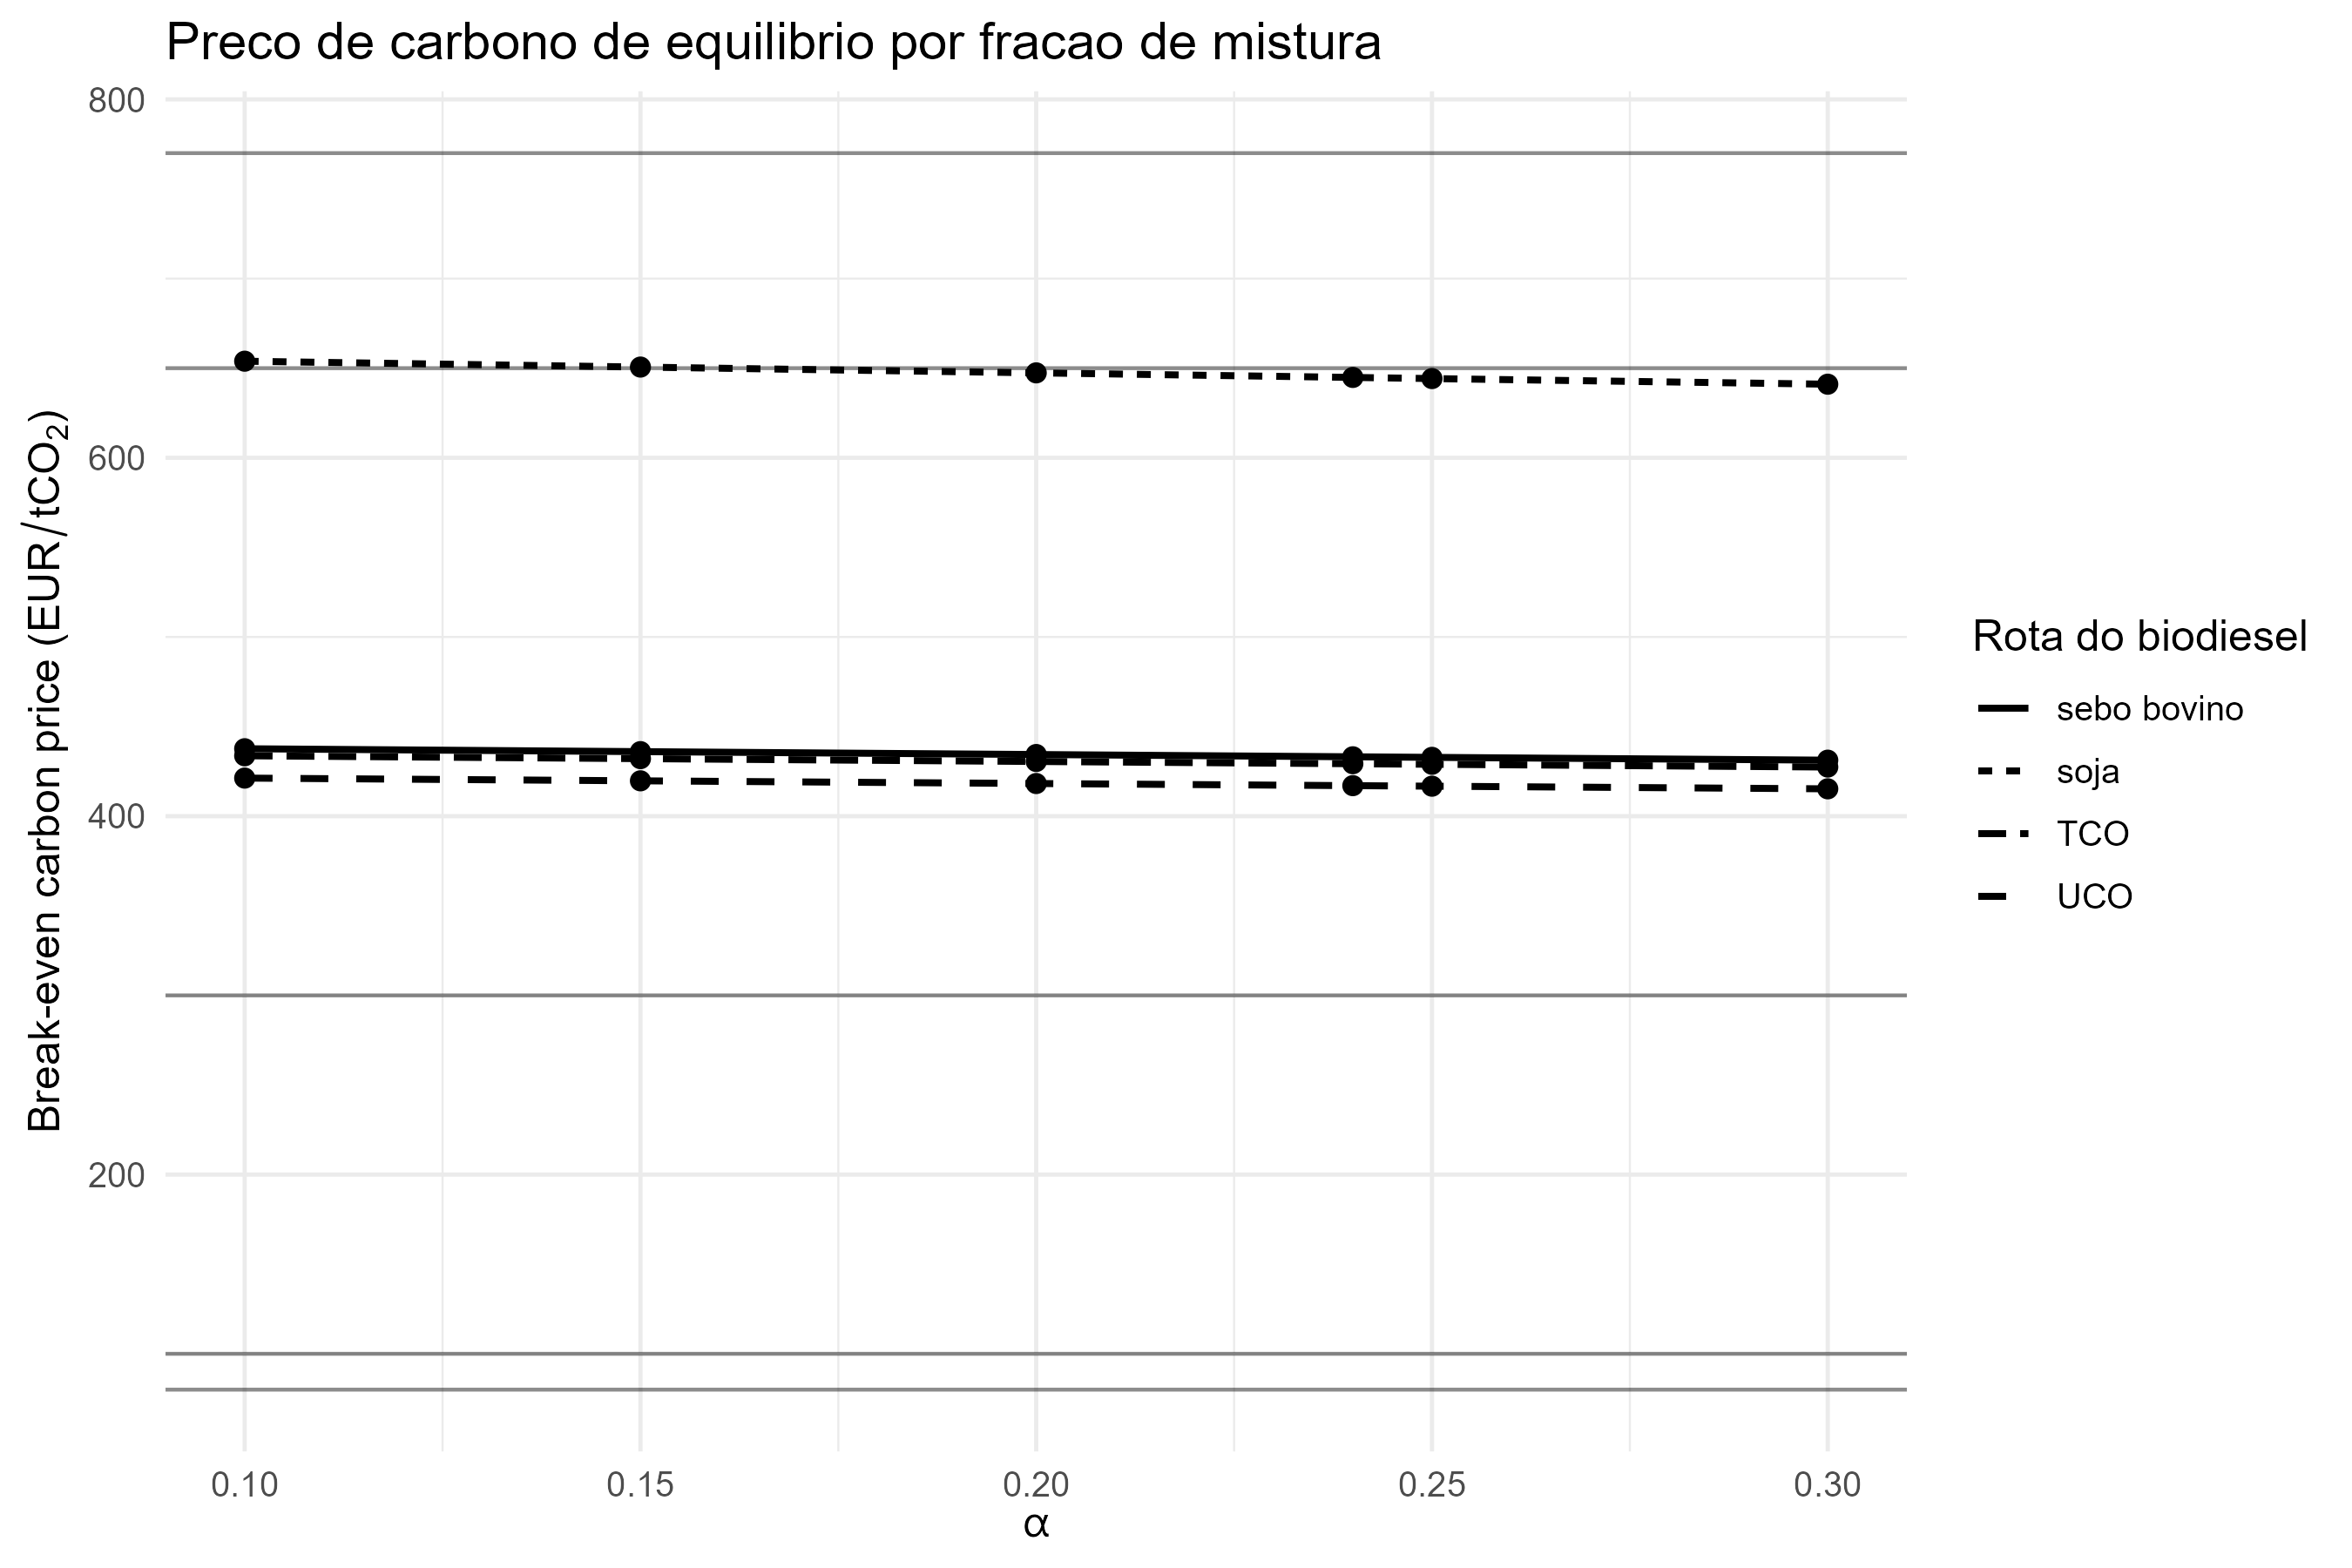
\includegraphics[width=0.85\textwidth]{grafico_03b_break_even_vs_alpha.png}
\caption{\warn{Preço de carbono de equilíbrio por fração de mistura e rota de biodiesel.}}
\label{fig:break_even_alpha}
\end{figure}

\warn{Os valores mínimos de preço de carbono de equilíbrio no cenário-base ocorrem em $\alpha = 0{,}30$ e são da ordem de $415,3\,\text{EUR}/tCO_2$ para \gls{UCO}, $427,4\,\text{EUR}/tCO_2$ para \gls{TCO}, $431,3\,\text{EUR}/tCO_2$ para sebo bovino e $641,1\,\text{EUR}/tCO_2$ para soja. Isso sugere que a atratividade relativa das rotas residuais ou de subprodutos industriais já se manifesta no modelo, mas ainda requer sinal regulatório mais forte do que o observado no mercado europeu de carbono, isto é, valores de $\gamma^{ref}$ significativamente superiores à faixa atualmente praticada no \gls{EUETS}.}

\warn{Em termos interpretativos, a Figura~\ref{fig:break_even_alpha} mostra mais do que uma simples ordenação entre rotas. Ela evidencia que o aumento de $\alpha$ melhora o desempenho relativo das alternativas renováveis no cenário-base, levando os menores preços de carbono de equilíbrio aos pontos de mistura mais altos testados. Isso indica que, na formulação atual, reduzir a fração renovável não é o caminho mais promissor para tornar o biobunker competitivo; ao contrário, as melhores condições econômicas relativas aparecem quando a mistura se aproxima do limite superior analisado.}

\begin{table}[!ht]
\centering
\caption{\warn{Preço de carbono de equilíbrio mínimo no cenário-base por rota de biodiesel}}
\label{tab:break_even_minimo}
\begin{tabular}{lccc}
\hline
\warn{Rota} & \warn{$\alpha$} & \warn{Break-even mínimo (EUR/tCO$_2$)} & \warn{Redução de emissões (\%)} \\
\hline
\warn{UCO} & \warn{0,30} & \warn{415,3} & \warn{21,6} \\
\warn{TCO} & \warn{0,30} & \warn{427,4} & \warn{21,5} \\
\warn{Sebo bovino} & \warn{0,30} & \warn{431,3} & \warn{20,8} \\
\warn{Soja} & \warn{0,30} & \warn{641,1} & \warn{14,0} \\
\hline
\end{tabular}
\end{table}

\warn{A Figura~\ref{fig:frontier_viabilidade} mostra a fronteira de viabilidade regulatória. Quando $\gamma^{ref}$ e $\gamma^{comp}$ são ampliados conjuntamente, os primeiros cenários viáveis aparecem a partir de aproximadamente $300\,\text{EUR}/tCO_2$, com destaque para \gls{UCO}, sebo bovino e \gls{TCO}. Para essas três rotas, as primeiras combinações viáveis ocorrem em torno de $\alpha = 0{,}24$, ao passo que a soja não se torna viável nem mesmo nos cenários regulatórios mais fortes testados.}

\warn{A utilidade desse gráfico está em transformar um resultado abstrato em fronteira observável de decisão. Em vez de afirmar apenas que determinados cenários ``não são viáveis'', a análise passa a mostrar em que patamar da família regulatória $\gamma$ a classificação muda. Isso permite interpretar a viabilidade como função conjunta de política climática, custo de \emph{compliance}, composição da mistura e, sobretudo, do nível de preço de carbono necessário para que o custo marginal de abatimento se torne compatível com o ambiente regulatório. No caso presente, a fronteira obtida indica que o \gls{EUETS} em níveis de mercado recentes é insuficiente, mas que regimes de indução mais fortes já colocam \gls{UCO}, sebo bovino e \gls{TCO} na região economicamente defensável.}

\begin{table}[!ht]
\centering
\caption{\warn{Primeiros cenários viáveis na exploração regulatória ampliada}}
\label{tab:primeiros_viaveis}
\begin{tabular}{lcccc}
\hline
\warn{Rota} & \warn{$\gamma^{ref}$ (EUR/tCO$_2$)} & \warn{$\gamma^{comp}$ (EUR/tCO$_2$)} & \warn{$\alpha$} & \warn{Redução (\%)} \\
\hline
\warn{UCO} & \warn{300} & \warn{300} & \warn{0,24} & \warn{17,1} \\
\warn{TCO} & \warn{300} & \warn{300} & \warn{0,24} & \warn{17,0} \\
\warn{Sebo bovino} & \warn{300} & \warn{300} & \warn{0,24} & \warn{16,5} \\
\warn{Soja} & \warn{--} & \warn{--} & \warn{--} & \warn{--} \\
\hline
\end{tabular}
\end{table}

\begin{figure}[!ht]
\centering
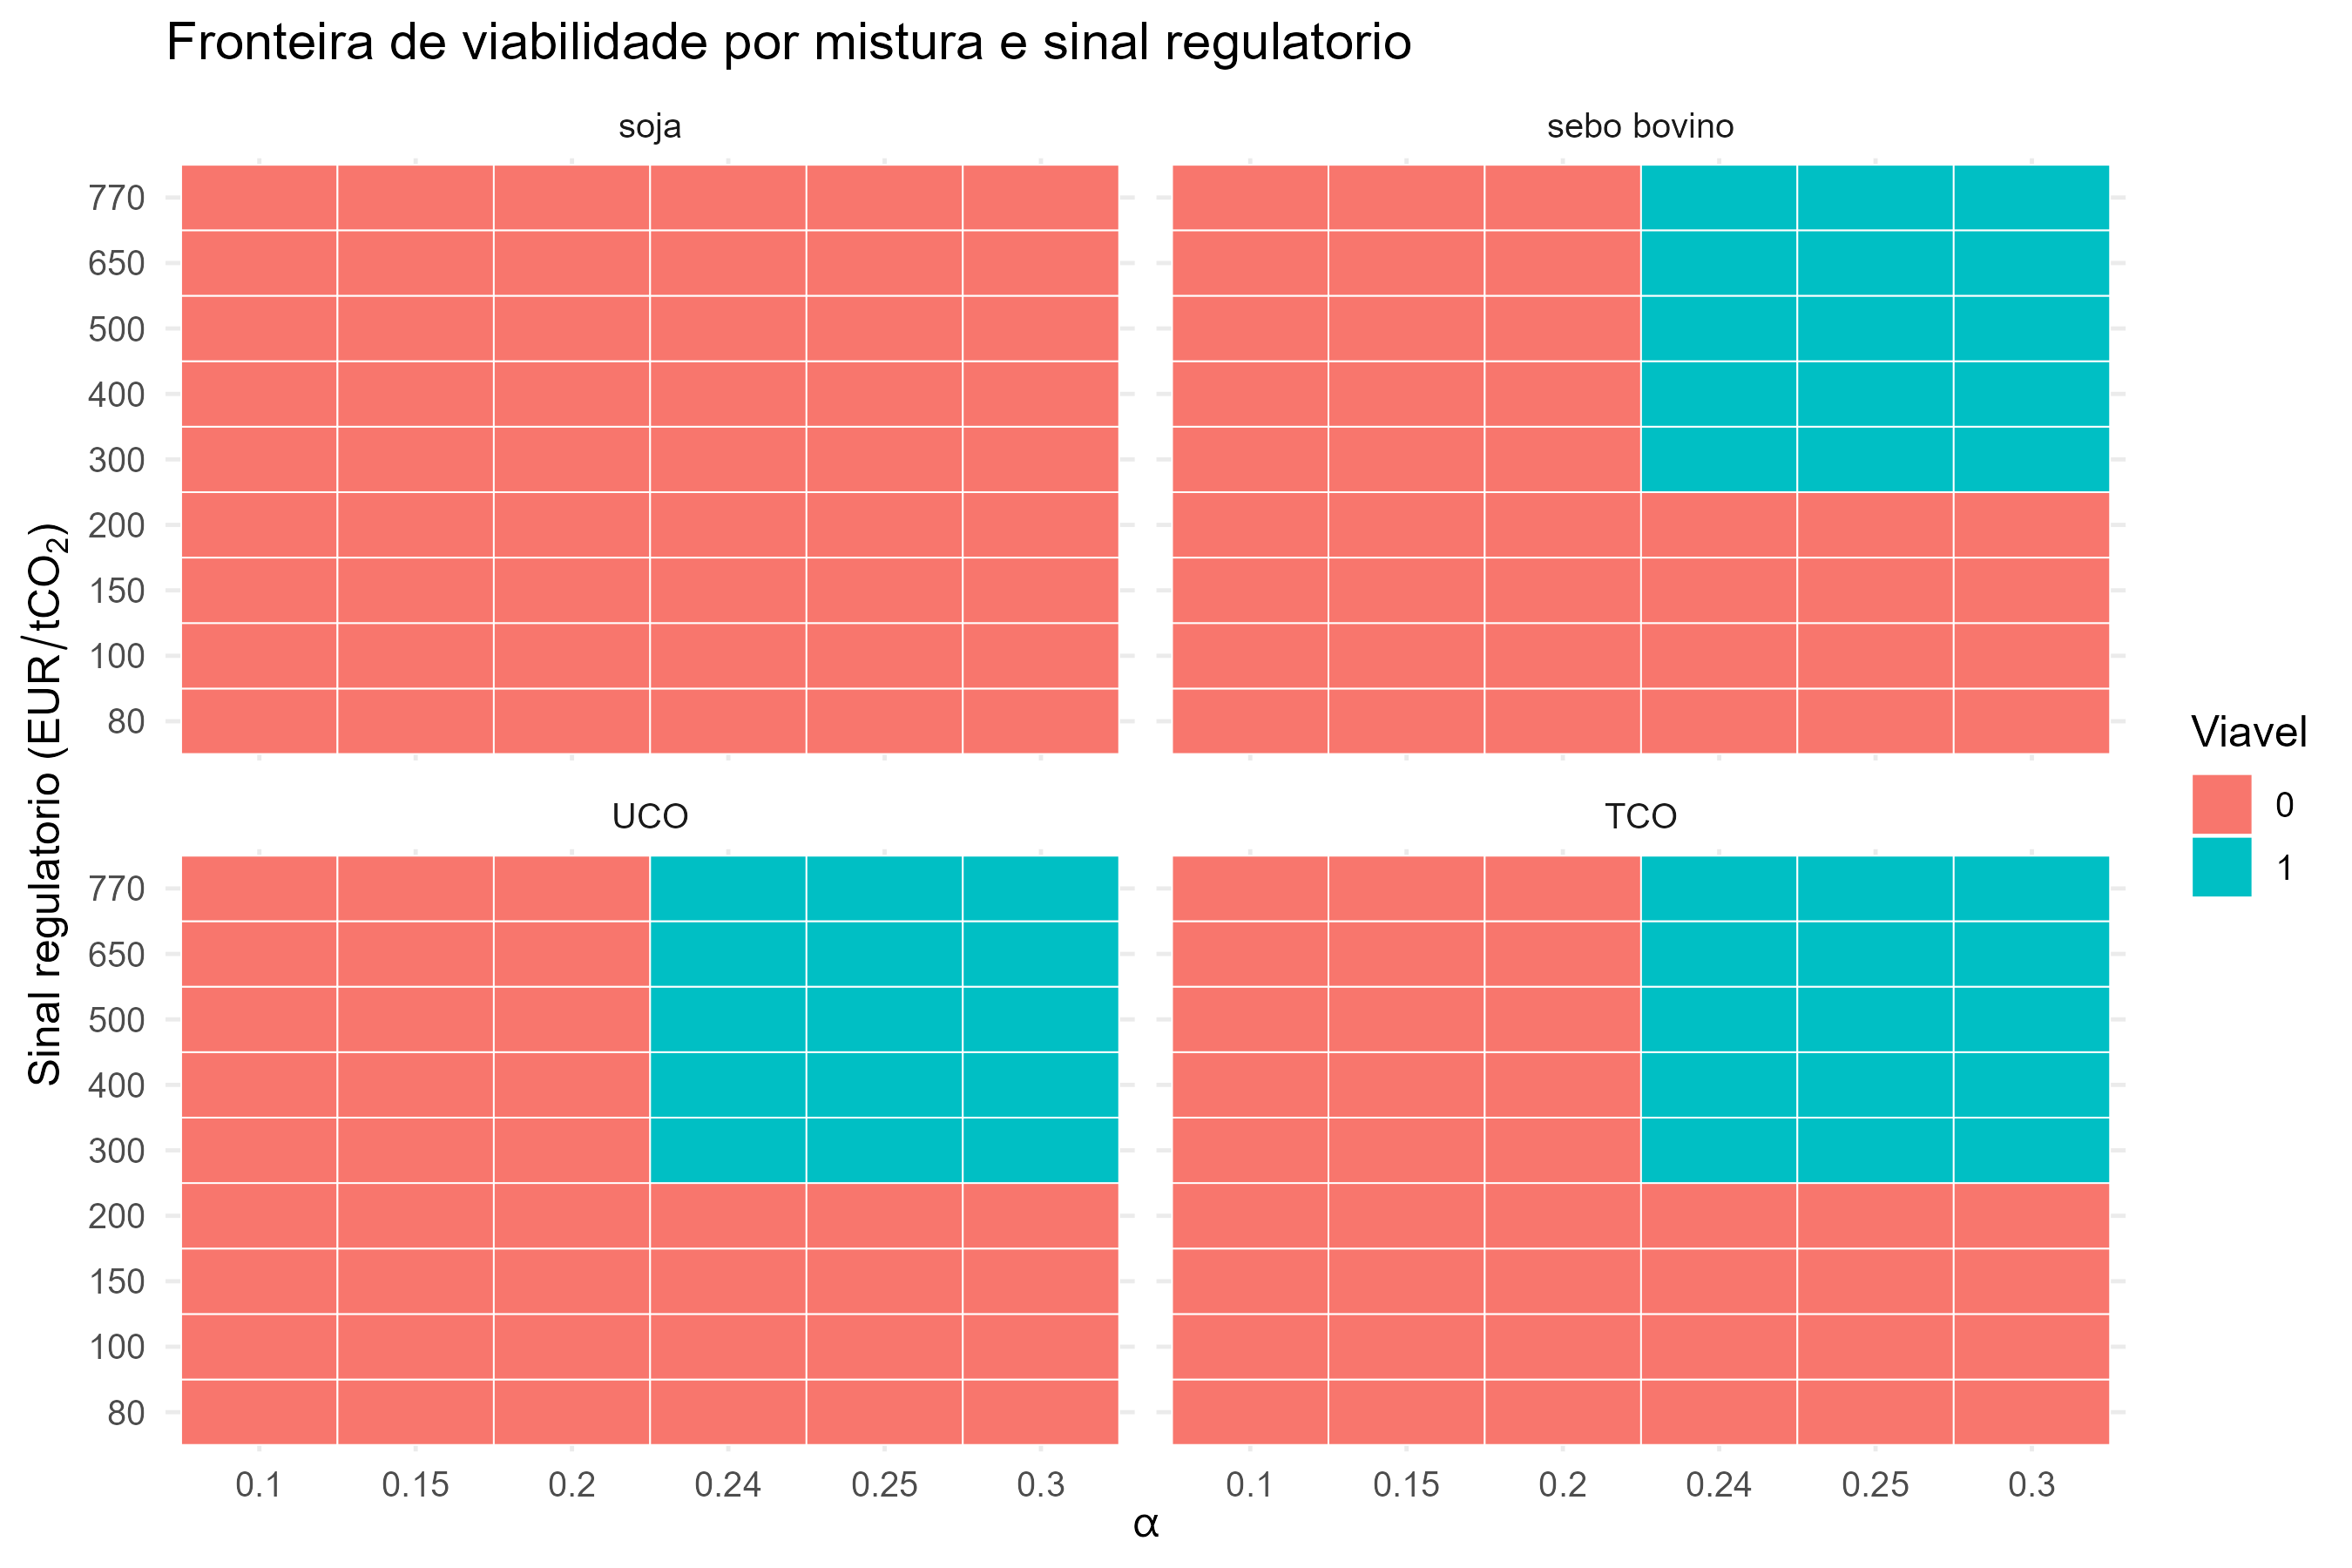
\includegraphics[width=0.95\textwidth]{grafico_07_fronteira_viabilidade.png}
\caption{\warn{Fronteira de viabilidade econômico-ambiental por fração de mistura, rota e sinal regulatório ampliado.}}
\label{fig:frontier_viabilidade}
\end{figure}

\warn{A leitura de custo também se altera quando o termo regulatório é explicitado. A Figura~\ref{fig:decomp_custo} decompõe o custo total entre combustível e a parcela de \emph{compliance} associada a $\gamma^{comp}$. Essa visualização evidencia que o custo regulatório cresce com a parcela fóssil remanescente, mas ainda não compensa, por si só, o diferencial de preço do biodiesel nos níveis correntes de mercado. Em outras palavras, o \gls{EUETS} melhora a competitividade relativa do biobunker, mas não basta sozinho para torná-lo viável sob os parâmetros-base.}

\warn{Esse ponto é importante porque evita uma leitura simplificada do papel da regulação. O componente $\gamma^{comp}$ atua como mecanismo de mitigação do diferencial econômico entre fóssil e biobunker, mas não elimina esse diferencial no nível atual de preços adotado na simulação. Assim, a análise preliminar sugere que a viabilidade depende menos de relaxar o critério ambiental e mais de combinar três alavancas: maior $\gamma^{ref}$, maior $\gamma^{comp}$, redução do preço relativo do biodiesel e escolha de rotas com menor intensidade de carbono, como \gls{UCO}, sebo bovino e \gls{TCO}.}

\begin{figure}[!ht]
\centering
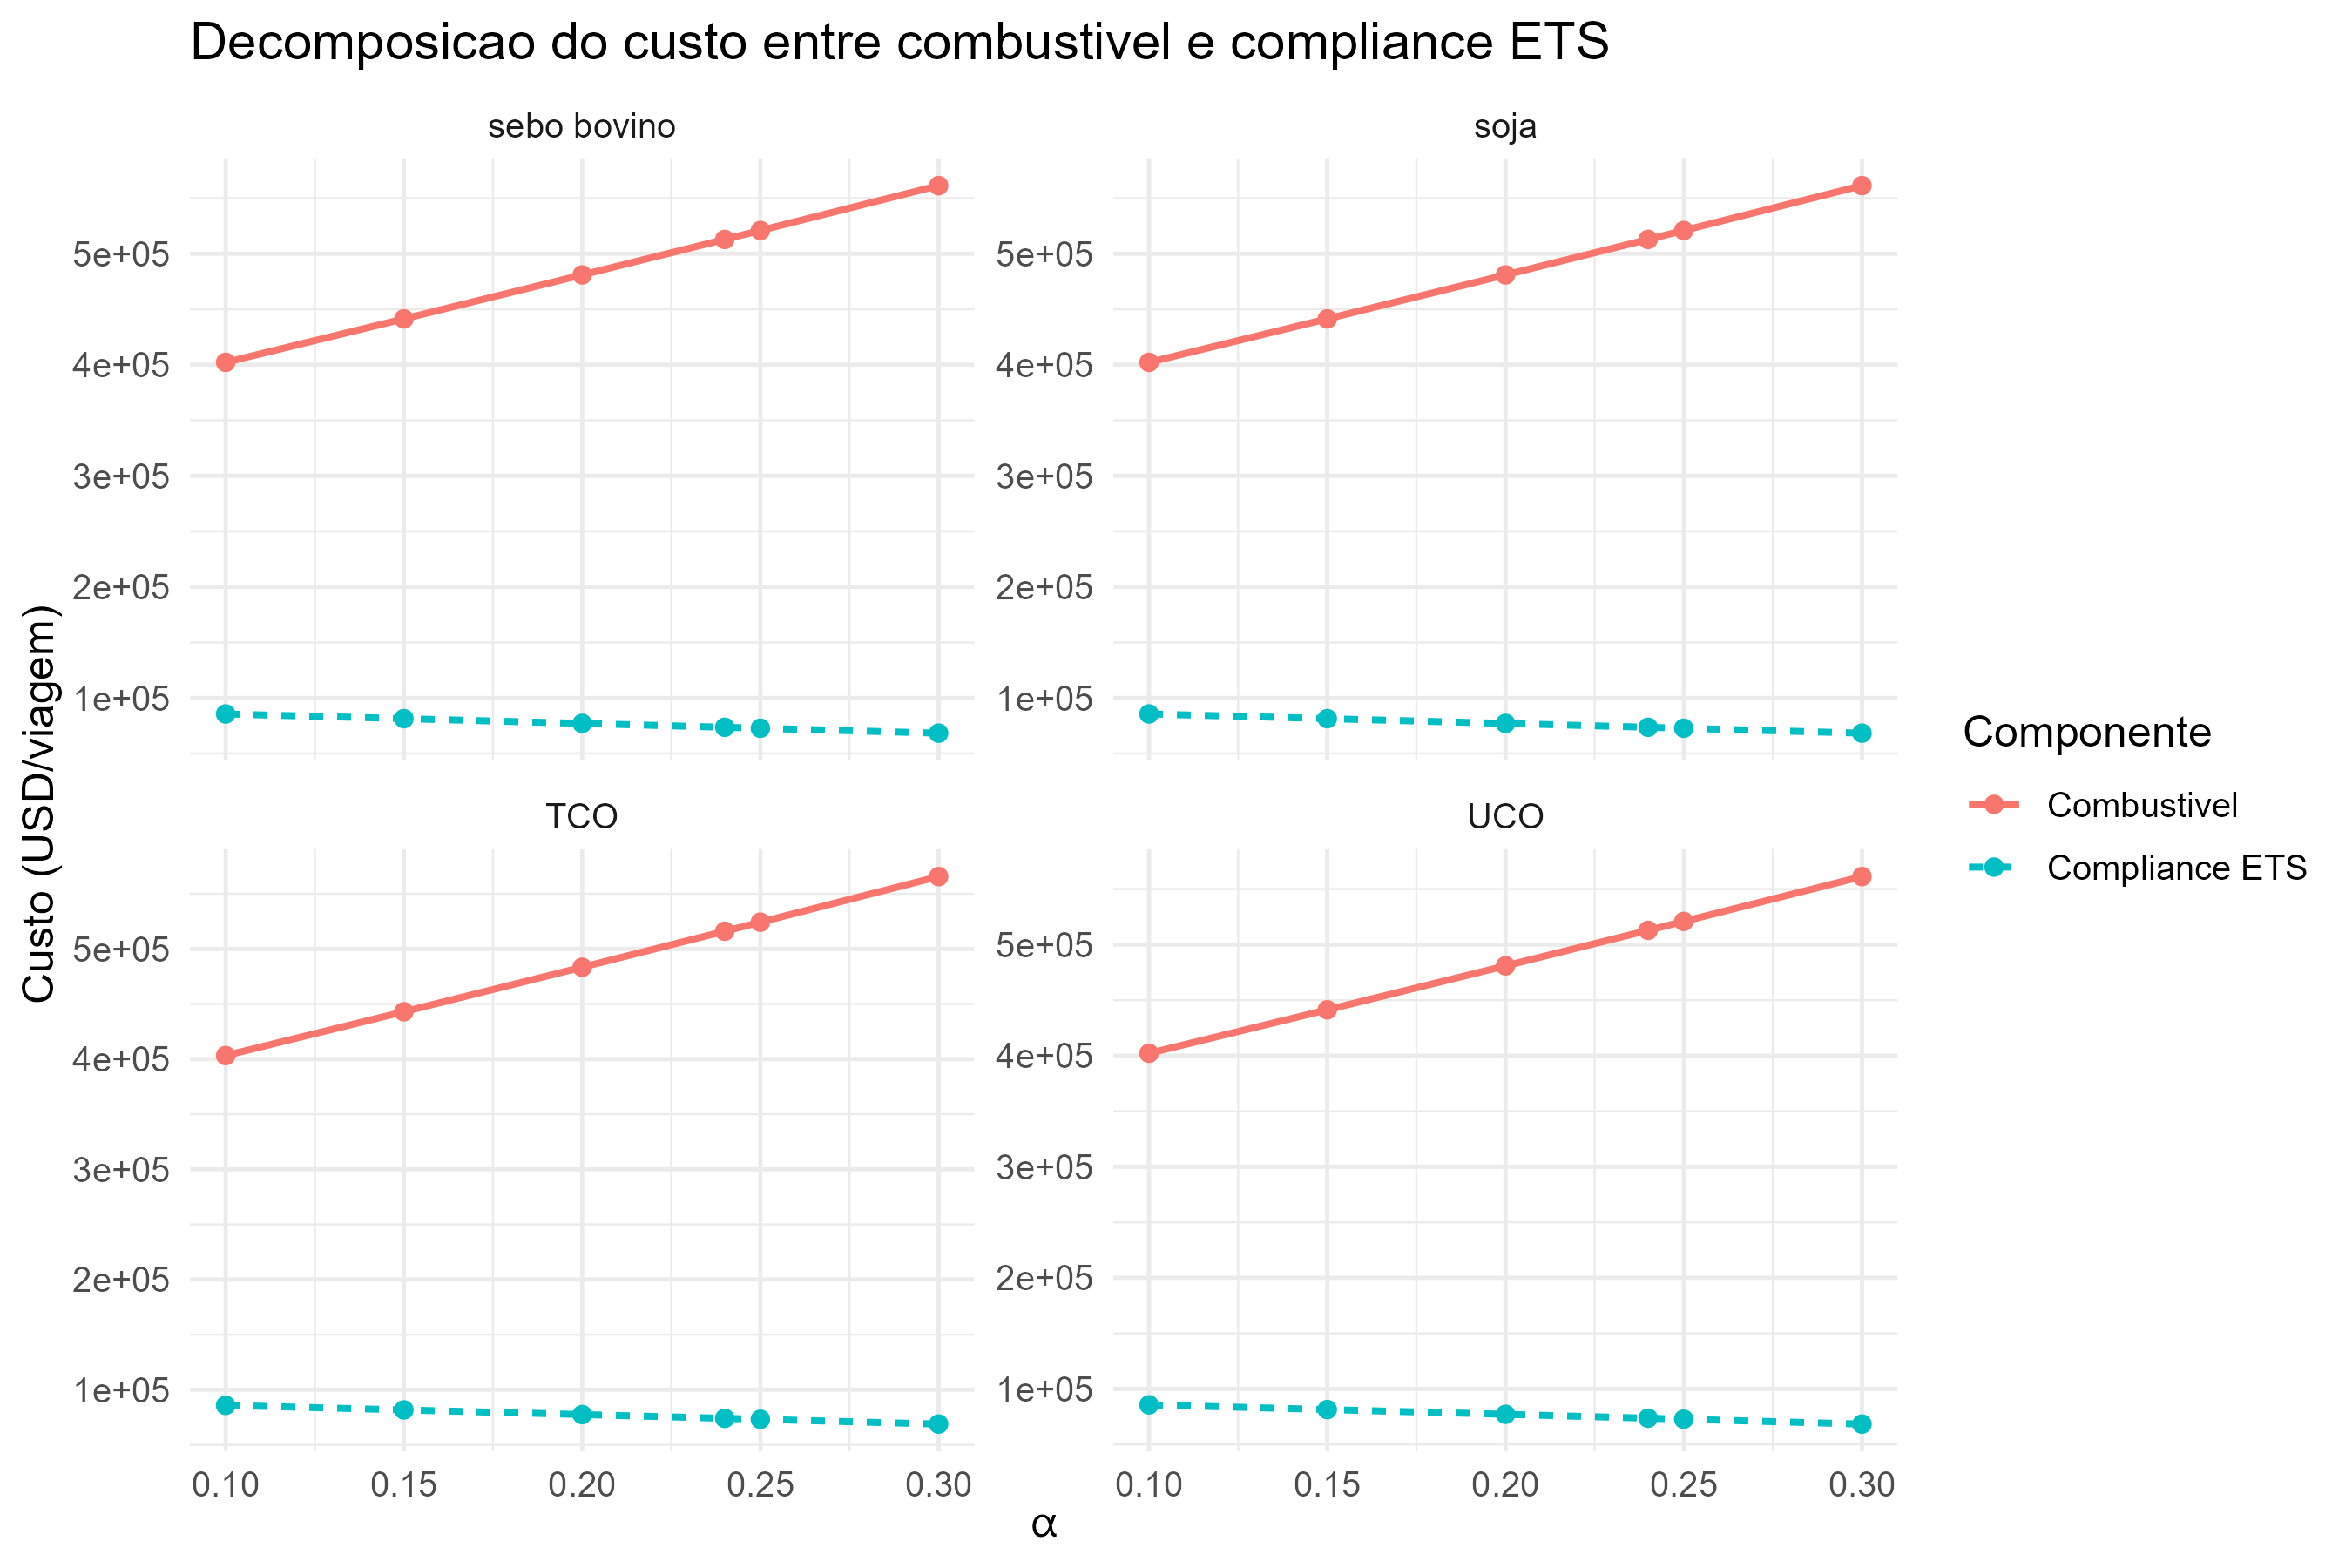
\includegraphics[width=0.95\textwidth]{grafico_06_decomposicao_custo.png}
\caption{\warn{Decomposição do custo total entre custo de combustível e custo de \emph{compliance} do \gls{EUETS}.}}
\label{fig:decomp_custo}
\end{figure}

\warn{No caso específico de \gls{TCO}, a análise preliminar indica desempenho próximo ao de \gls{UCO} e sebo bovino quando se utilizam os parâmetros-base. Entretanto, a sensibilidade específica dessa rota mostra que sua atratividade depende de forma relevante do fator de emissão \gls{WTW} e, sobretudo, do preço relativo do biodiesel produzido a partir desse subproduto. Essa evidência reforça a necessidade de tratar \gls{TCO} como rota promissora, porém mais sensível a escolhas metodológicas e econômicas do que as rotas residuais mais consolidadas.}

\warn{Em síntese, os resultados preliminares apontam três conclusões centrais}. \warn{Primeiro, o custo marginal de abatimento dos cenários avaliados permanece acima do intervalo de referência $\gamma^{ref}$ sob condições atuais, caracterizando inviabilidade econômica-regulatória.} \warn{Primeiro, a inviabilidade do biobunker sob sinal regulatório de carbono na faixa recente do \gls{EUETS}. Segundo, a emergência de cenários viáveis para \gls{UCO}, sebo bovino e \gls{TCO} quando se simulam regimes de indução regulatória mais fortes. Terceiro, a utilidade analítica do preço de carbono de equilíbrio como métrica-síntese para comparar rotas, frações de mistura e condições regulatórias em um mesmo quadro interpretativo.}
